\documentclass[a4paper]{article}
\usepackage[a4paper,
            bindingoffset=0.2in,
            left=1in,
            right=1in,
            top=1in,
            bottom=1in,
            footskip=.25in]{geometry}

\usepackage{amsmath}

\usepackage{graphicx}

\usepackage{hyperref}
\usepackage{hyphenat}
\usepackage{enumitem}
\usepackage[yyyymmdd]{datetime}
\usepackage{caption}

\usepackage[utf8]{inputenc}
\usepackage{microtype}

\usepackage[sorting=none, backend=biber]{biblatex} %Imports biblatex package

\addbibresource{whitepaper.bib} %Import the bibliography file

\captionsetup{justification=centering,width=0.7\textwidth}


\newdateformat{UKvardate}{%
\THEDAY\ \monthname[\THEMONTH], \THEYEAR}
\UKvardate

\providecommand{\keywords}[1]
{
  \small	
  \noindent\textbf{\textit{Keywords---}} #1
}

\providecommand{\purpose}[1]
{
  \small
  
  \textbf{This paper will:} 
  #1
}

\sloppy

\begin{document}

\title{Jackal Protocol: A Next Generation Data Storage Network and Decentralized Application Protocol}

\author{Jackal Labs}

\date{\today}


\maketitle


\begin{abstract}
Citizens of the internet should possess fundamental human rights, including the right to data security and privacy, without sacrificing a great user experience. This is possible with blockchain and peer-to-peer technology. In recent years there has been great success in open-source blockchain ecosystems such as Cosmos Hub, Ethereum, Near Protocol, Avalanche, Algorand, and Polkadot. These ecosystems share the vision of a decentralized internet with permissionless and algorithmic applications, yet this technology lacks on-chain data storage capacity greater than 1kb at scale with smart contracts. Although they strive for decentralized and permissionless products, these applications are often forced to incorporate centralized data storage providers and middleware, a cyber security and digital privacy attack vector. This is often the cause of disruptions to blockchain applications-centralized data center outages and domain name service hijacking. Current decentralized data storage solutions have gross insufficiencies, limited performance, and an inefficient user experience with a lack of security and privacy.

The Jackal Protocol is a fast, scalable, and secure blockchain that empowers individuals, developers, and enterprises to increase their data privacy and cybersecurity posture without sacrificing ease of use. The protocol strives to offer world-class applications to protect the planet's most important data-your data. Jackal is a distributed and decentralized network that combines: the data capacity of a legacy cloud storage solution, the ownership of digital assets using ledger technology, the flexibility of smart contracts, and the speed of Byzantine fault-tolerant consensus. Data stored on the protocol is self-custodial, meaning that only the end-user with their private key can view, access, and share their files. No one-not even the team at Jackal Labs-can access or view your data.  Unlike other blockchains, the Jackal Protocol has both Validators and Storage Providers. Validators are incentivized to verify transactions and secure the Jackal Protocol, while Storage Providers are incentivized to warehouse Jackal Protocol users' encrypted and distributed data.  The Protocol is powered by the Jackal Utility Token (called JKL), which provides incentives to the network in various ways.
\end{abstract}

\purpose{
\begin{enumerate}
    \item Introduce the Jackal Protocol and provide an overview of the blockchain, including each genesis blockchain module and its application. 
    \item Introduce the Jackal Token (JKL) and its utility throughout the Jackal Protocol and surrounding ecosystem. 
    \item Formalize the Jackal Proof-of-Persistence (JPOP) algorithm and its implementation within the Jackal Storage blockchain module. 
    \item Discuss how to use the Jackal Protocol, its use cases, interoperability within the Cosmos Ecosystem, and interoperability with other blockchain ecosystems. 
\end{enumerate}
}

\keywords{Decentralized Data Storage, Proof of Persistence, Tendermint, Cosmos SDK, Blockchain, Jackal Protocol, Decentralized Applications}

\newpage
\tableofcontents
\newpage

\section{Introduction}
The Jackal Protocol is a fast, scalable, and secure blockchain that empowers individuals, developers, and enterprises to increase their data privacy and cybersecurity posture without sacrificing ease of use. The protocol strives to offer and support world-class applications to protect user data. 

Unlike other blockchains, the Jackal Protocol utilizes both validators and storage providers. The Jackal Protocol allows developers to build decentralized applications with the ability to interface with all Jackal Protocol Modules-including storage contracts and file structure. This grants developers the ability to adjust the ownership of data, share data with other jackal users or smart contracts, and transfer small or large amounts of encrypted data without centralized storage providers or middleware. Data on the Protocol is always self-custodial, meaning no one- not even the team at Jackal-can access or view user data. 
\section{Motivation}
Before the Jackal Protocol, there was KeepSake, a digital evidence capture, chain of custody management, and e-discovery tool. The team believed we could build the next generation of e-discovery software for legal teams with higher security and verifiability using blockchain technology. However, we quickly realized a glaring roadblock-no storage layer could store data in a clean forensic environment effectively, privately, securely, and at scale on the decentralized web. This was the motivation to build a generalized data storage solution with the highest digital privacy and cybersecurity posture possible without sacrificing ease of use. 

\section{Technology Stack}
\subsection{Tendermint Consesus}
Tendermint is a partially synchronous Byzantine fault-tolerant (BFT) consensus protocol built by Jae Kwon and Ethan Buchman. The protocol requires a fixed, known set of validators, where their public key identifies each validator. Validators attempt to come to a consensus on one block at a time, where a block is a list of transactions. Voting for consensus on a block proceeds in rounds. Each round has a round leader, or proposer, who proposes a block. The validators then vote, in stages, on whether to accept the proposed block or move on to the next round. The proposer for a round is chosen deterministically from the ordered list of validators in proportion to their voting power. The security Tendermint is derived from optimal Byzantine fault tolerance through super-majority voting and a locking mechanism. \cite{tendermint}
\subsection{CosmosSDK}
The Cosmos SDK is an open-source framework for building custom application-specific blockchains that can natively interoperate with other blockchains built on Tendermint. The Jackal Protocol uses the Cosmos SDK due to the composability of blockchain modules, where we can add and alter these modules for our application-specific needs. \cite{cosmossdk}
\subsection{Encryption}
Jackal has two main features that rely on encryption techniques to keep user data private and secure. The two main models are file encryption and file-entry encryption. These reside in different locations within the protocol. The files themselves are stored on Storage Providers, which require files to be encrypted before they are transferred to those machines. The file entries are data structures living directly on-chain in the File Tree blockchain module, again needing to be encrypted on the client's device before being sent to the blockchain. The file encryption model is simply performed by taking the file as raw bytes and randomly generating a key in the user's client. This key is called a Symmetric Key. We then pass both the key and the file through AES256 encryption, which results in an encrypted file that can safely be sent to the Storage-Providers.
\begin{figure}[!htbp]
\centering
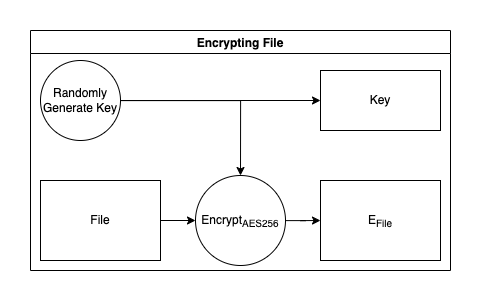
\includegraphics[width=0.8\textwidth]{assets/enc1.png}
\caption{Example of generating a symmetric key and encrypting a file}
\end{figure}

What is done with this key is equally important as the encryption performed on the file; if the key were made public, all encryption on the file itself would be naught. Therefore, we need to store this key somewhere safe and immutable. This safe place is the Jackal Chain, specifically the File Tree Module. The key is stored in the encrypted form alongside the file's location to make mapping each key to its respective file easy. To get this key into its encrypted form, we use an Integrated Encryption Scheme based on AES and the Elliptic Curve used to generate Bech32 Addresses \cite{bech32}. To do this, the protocol takes a user's public key and encrypts the private key with it.

\begin{figure}[!htbp]
\centering
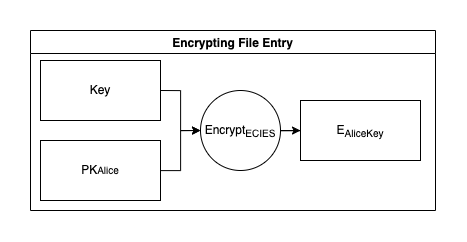
\includegraphics[width=0.8\textwidth]{assets/enc2.png}
\caption{Example of encrypting a symmetric key with a users public key}
\end{figure}


After this, the protocol ends up with an encrypted key that only the user whose public key was used can decrypt. When looking to decrypt a file, the process is reversed and instead uses the user's private key to decrypt the symmetric key. Following the retrieval of the symmetric key, we can decrypt the file stored on the Storage-Providers, leaving us with the originally uploaded file.

\begin{figure}[!htbp]
\centering
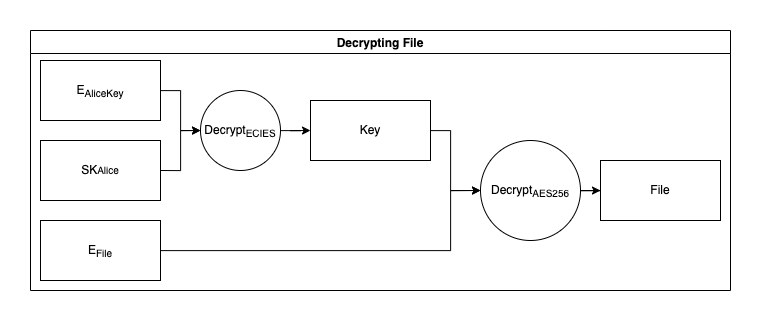
\includegraphics[width=0.9\textwidth]{assets/enc3.png}
\caption{Example of fully decrypting a file}
\end{figure}

When sharing files, we can semi-repeat this process by first decrypting the key from the chain. Then we can grab the public key of an external user from the chain itself and encrypt the files with that key instead of our own. Finally, we append the newly encrypted symmetric key to the file entry giving that user access to the key.

\section{Jackal Proof of Persistence (JPOP)}
\subsection{Intro}
Jackal Storage functions by a Proof-of-Storage algorithm we call Proof-of-Persistence. The Jackal Proof-of-Persistence (JPOP) works through a series of contracts between the storage provider and the user. These contracts contain the Merkle Tree root hash of the file and the information required to prove ownership of the file. Storage Providers are responsible for posting Merkle Proofs within a challenge window determined by the blockchain. These challenge windows need the provider to post the raw chunk of data corresponding to the index of the challenge window alongside the required Merkle Hashes to prove the data belongs to the Merkle Root stored on the contract. These challenge indexes are chosen randomly by the blockchain using a block-hash-based random number generator paired with a random data oracle.
If a Storage Provider successfully posts a Merkle Proof within the challenge window for the contract and the Validators verify the data to be valid Merkle Proofs for the challenge index, the Storage Provider is rewarded. Storage Provider rewards are proportional to the file size the contract is associated with relative to every other active contract on the network. If a Storage Provider fails to provide a valid proof within the allotted time frame, the contract is struck with a missed proof. After X missed proofs, the contract is burned, and the User is alerted the next time they query the contract. For every contract burned through missing proofs, the Storage Provider is struck with a penalty that remains on their record for a period of time adjustable through governance.
\subsection{Building the Trees}
Merkle Trees are a core component of the JPOP mechanism; thus, it is important to outline how these trees are used to create efficient and trustworthy proofs. When saving a file for the first time, providers split each file into 1kb chunks. Providers must also hash the entire file to create a folder to house every chunk, the following diagram displays this.
\begin{figure}[!htbp]
\centering
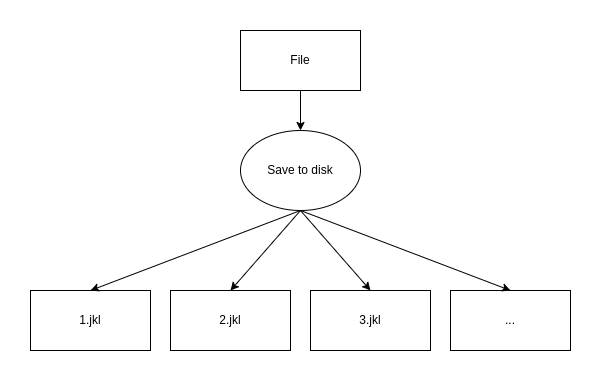
\includegraphics[width=0.7\textwidth]{assets/tree1.png}
\caption{Example of a file representation on disk}
\end{figure}

\begin{figure}[!htbp]
\centering
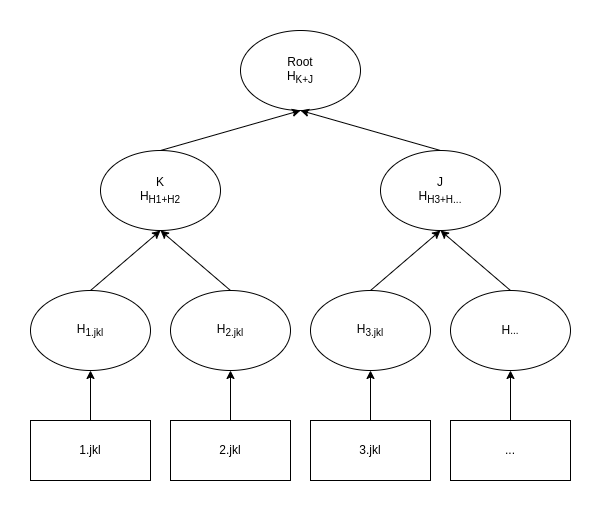
\includegraphics[width=0.7\textwidth]{assets/tree2.png}
\caption{Example of a Merkle Tree built from the file on disk}
\label{fig:tree2}
\end{figure}

These chunks are used as leaves on the Merkle Tree defining each storage contract. Immediately after saving a file to disk, the storage provider builds a tree using each chunk. To create this tree, each chunk is hashed into a respective Hashed Chunk. These chunks are then recursively paired together and hashed until a single root node is created. This is called the Merkle Root, the only piece of data relative to a file that is saved directly on the blockchain itself. Figure \ref{fig:tree2} displays how each file is hashed together to create a single root node.

\newpage
\subsection{Prooving Data Availability}
These nodes are essential as they only require the nodes below them to prove they are part of the tree. This means we can create a proof claiming a single chunk belongs to the file using the Merkle Root saved on the blockchain. In the following diagram, only the blue nodes are required to build a successful proof. The green nodes represent information that can be generated given the blue nodes. Finally, we can compare the root generated from the proof to the root saved on the chain and determine if the chunk does belong to the contract we are proving. This results in small message sizes due to not needing to send the entire file every proof.
\begin{figure}[!htbp]
\centering
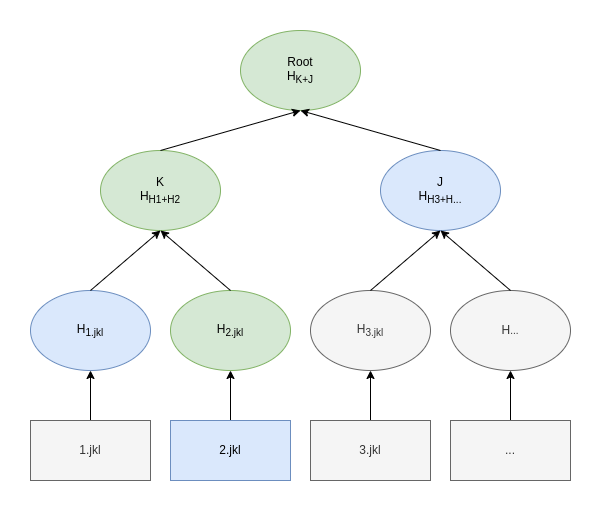
\includegraphics[width=0.7\textwidth]{assets/tree3.png}
\caption{Example of the minimal requirements to prove a node belongs to a tree}
\end{figure}

\newpage
\section{Protocol}

\begin{figure}[!htbp]
\centering
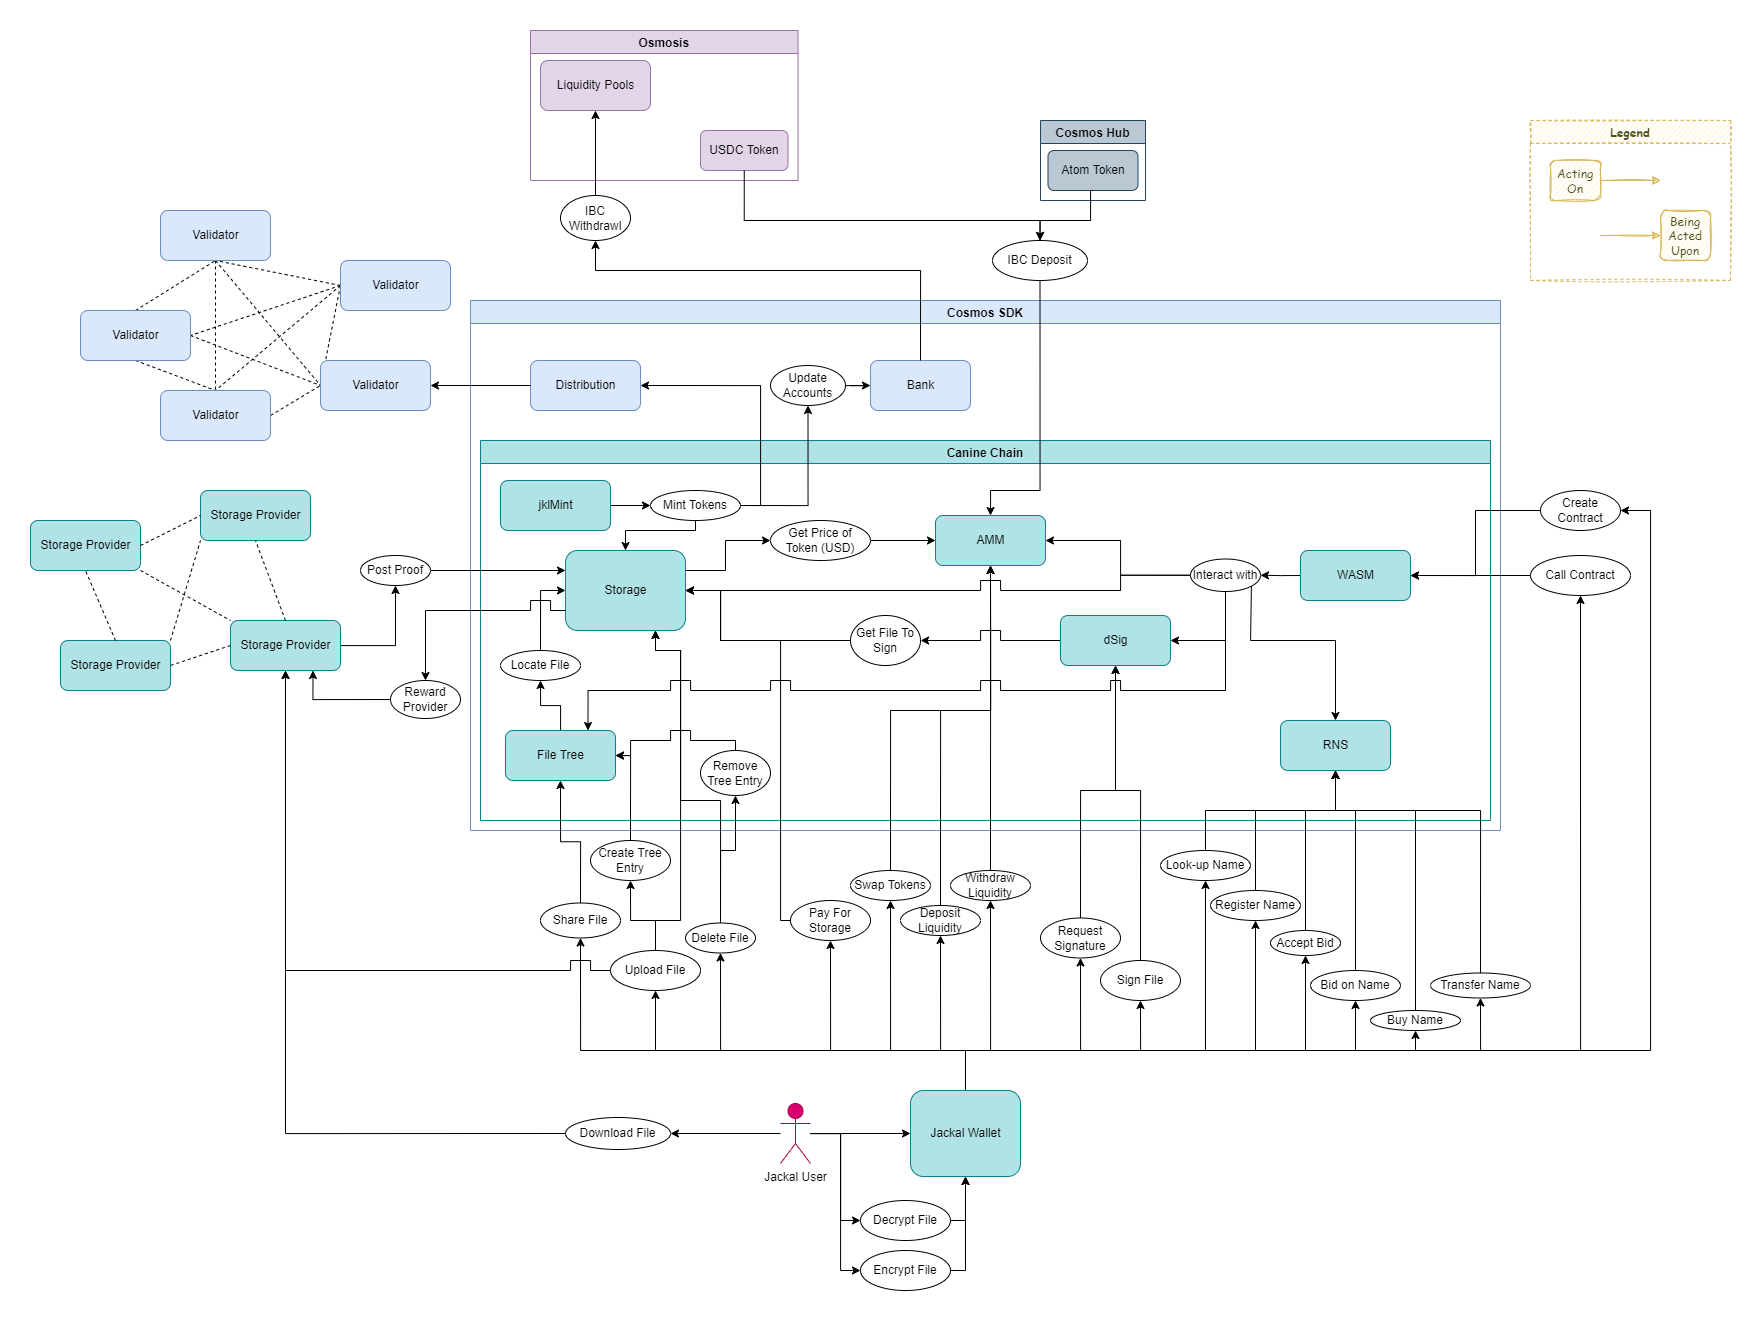
\includegraphics[width=1\textwidth]{assets/protocol.png}
\caption{The entire Jackal Protocol overview}
\end{figure}

The Jackal Protocol consists of seven modules, two tokens, dedicated validators, and dedicated storage providers. The modules include jklmint, lp, rns, wasm, storage, dsig, and filetree. The tokens include JKL and JWL.  These modules and tokens can be united in various ways to create secure, scalable, and decentralized applications. Users of these decentralized applications interact with the chain and each other through public and private encryption keys.

\newpage
\subsection{Modules}
\subsubsection{jklmint}
The jklmint module is a replacement for the Cosmos-SDK module: Mint \cite{mint}. The key differences between this and the pre-existing minting module are that jklmint does not adjust inflation based on the rate of bonded tokens. At genesis, the jklmint module produces 10 JKL per block and distributes it to both the storage module and the default distribution module.

\begin{figure}[!htbp]
\centering
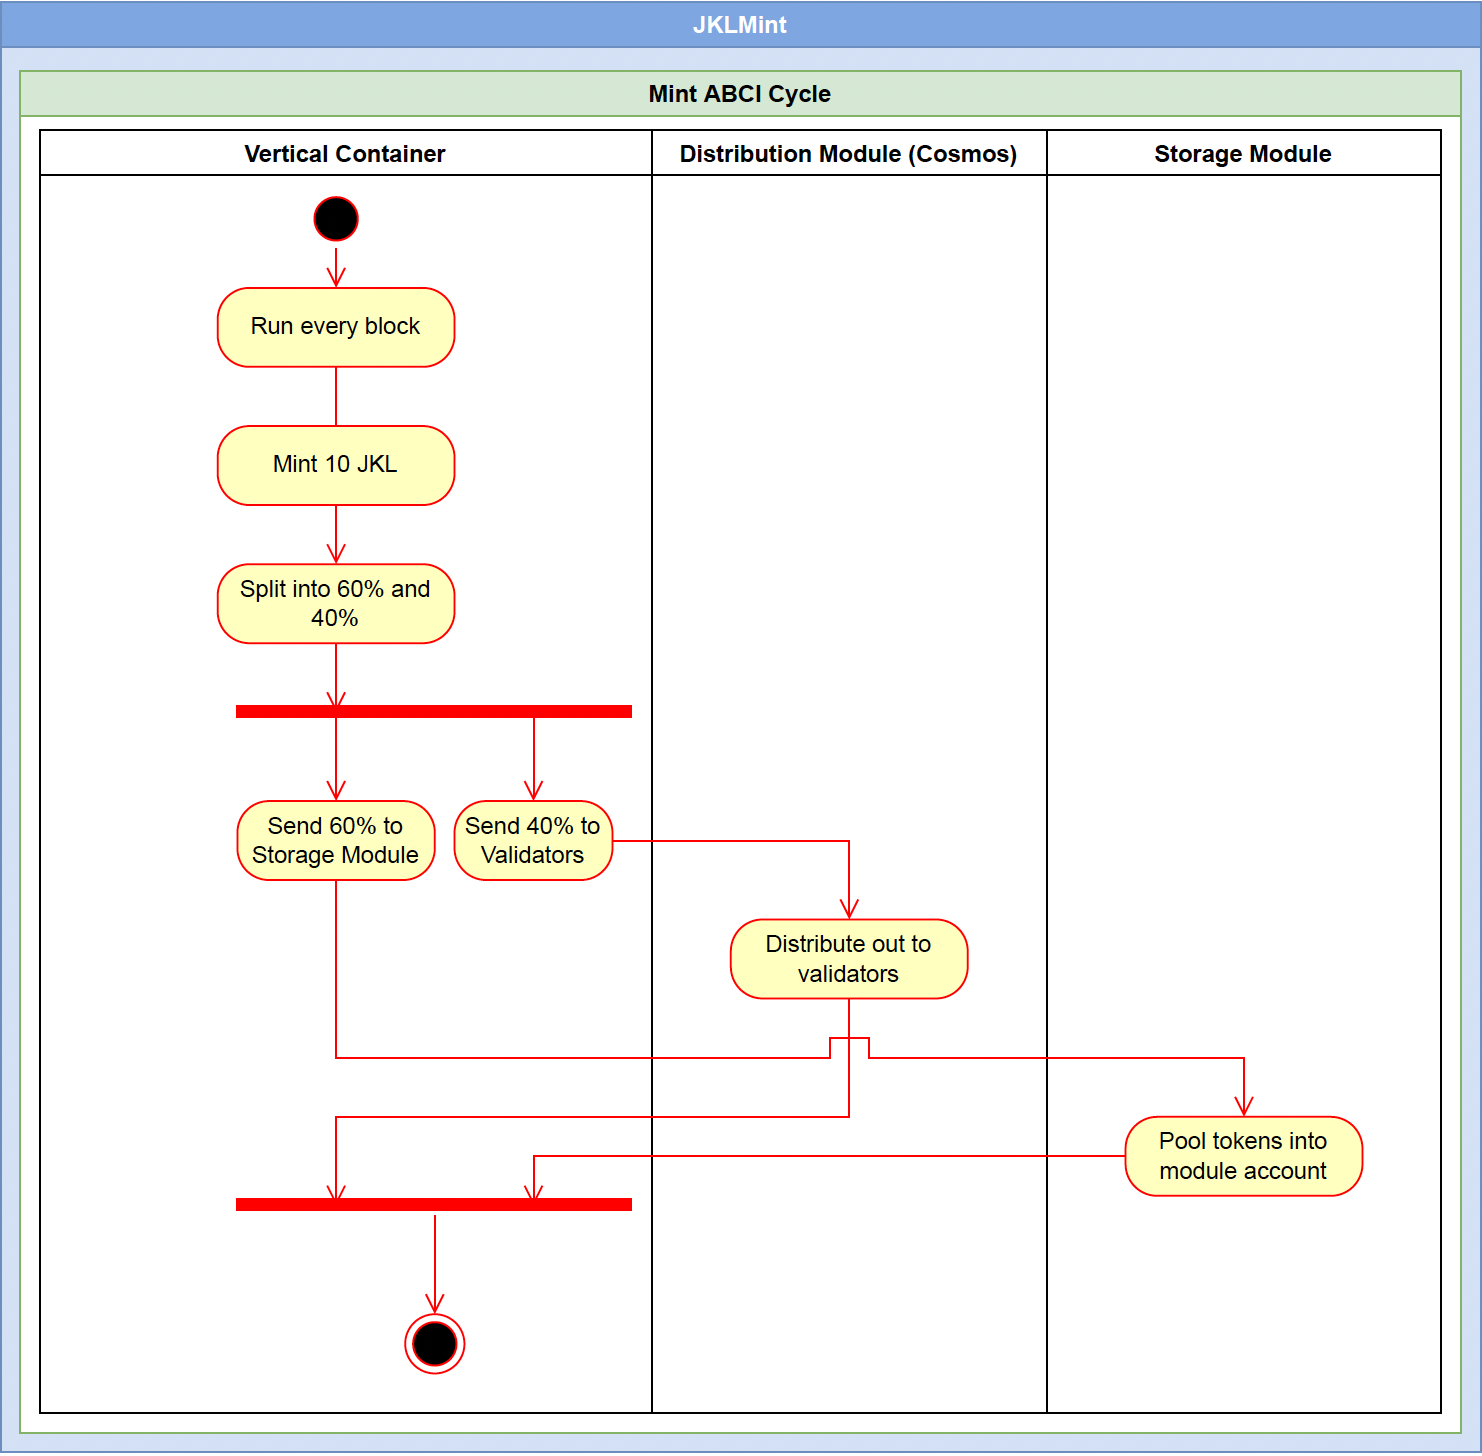
\includegraphics[width=0.7\textwidth]{assets/mint.png}
\caption{}
\end{figure}

\newpage

\subsubsection{LP}
The lp module allows for a native automated market maker (AMM) liquidity pools (LP) to be built directly into the Jackal Blockchain. This allows for local prices for payment mechanisms without the need for price oracles, along with the ability to swap tokens directly from the Jackal dashboard, Jackal Swap app, and wallet. 


\begin{figure}[!htbp]
\centering
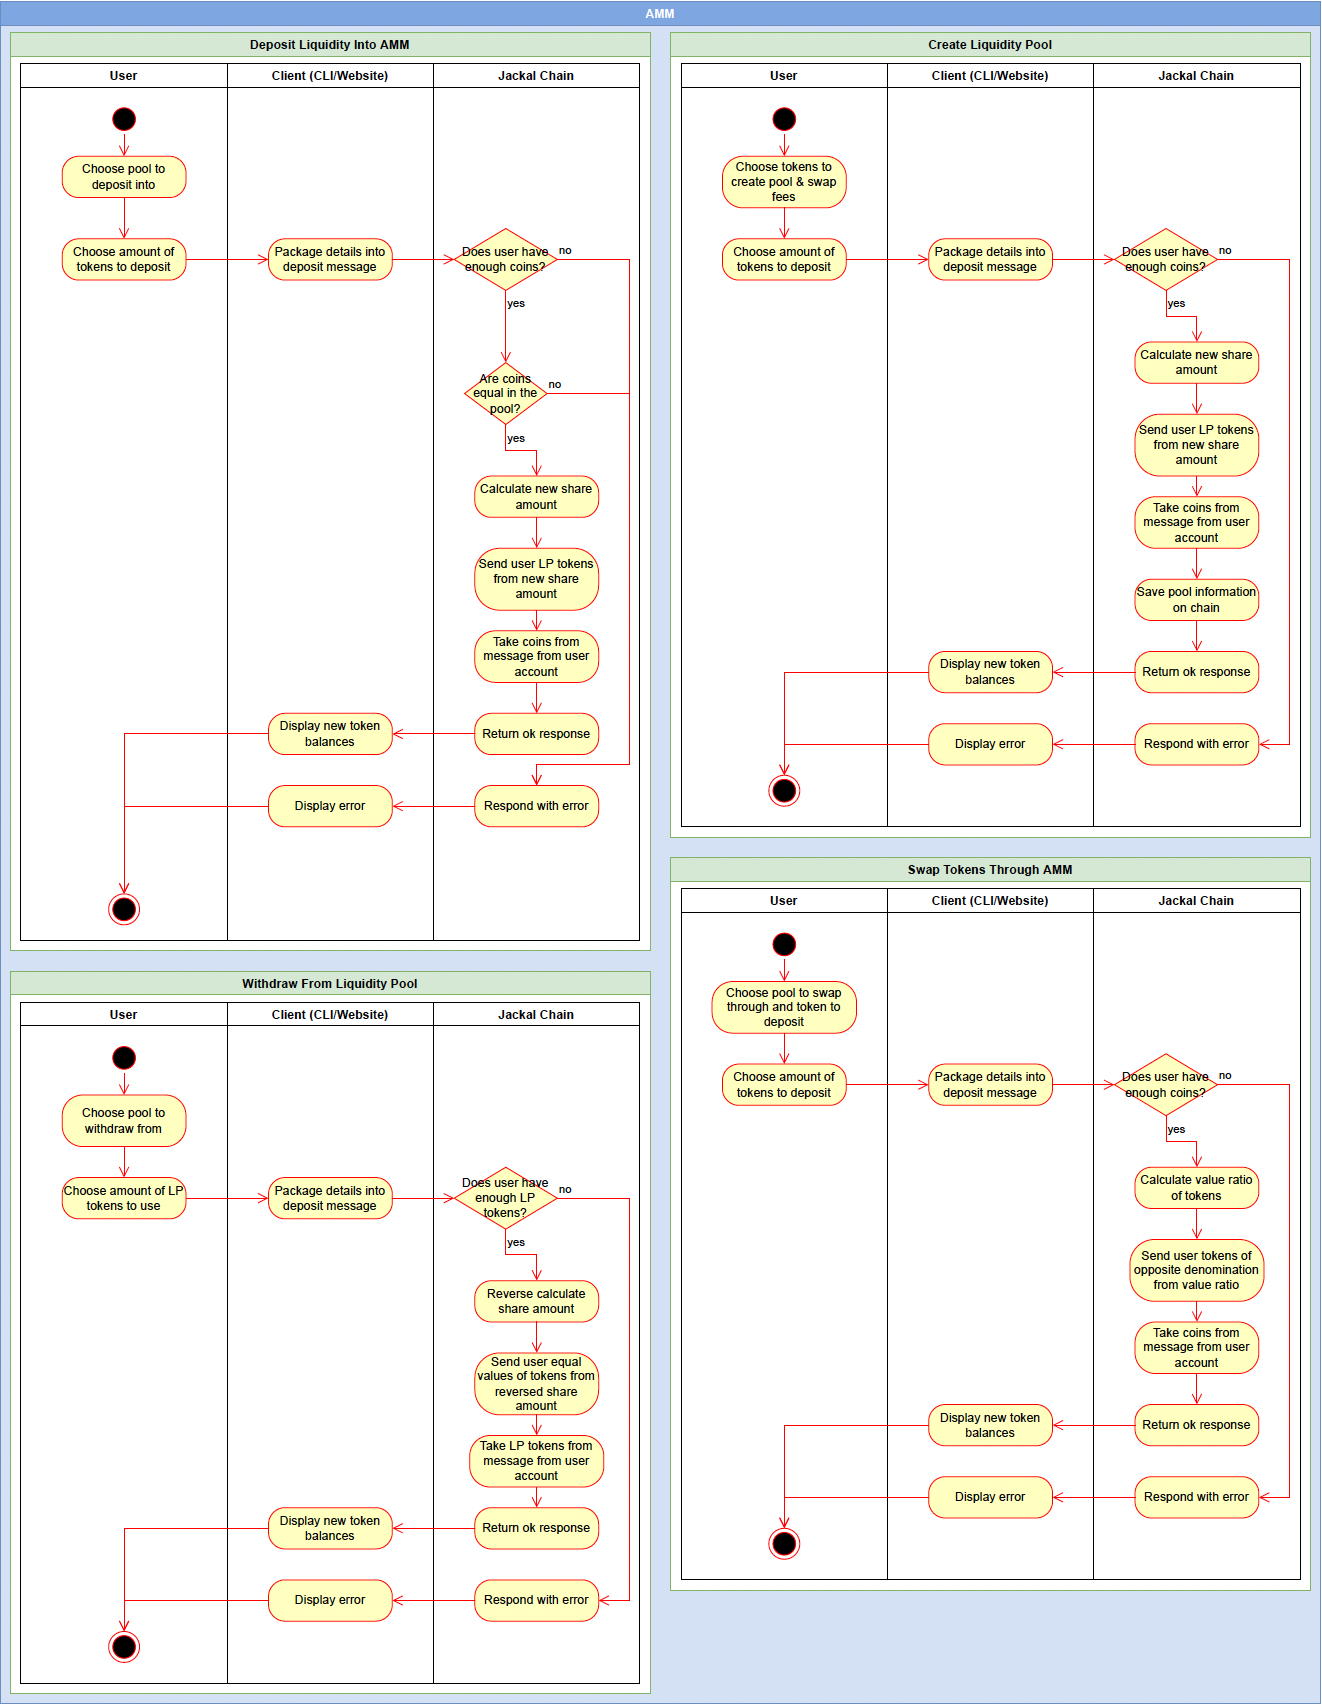
\includegraphics[width=0.7\textwidth]{assets/lp1.png}
\caption{}
\end{figure}

\begin{figure}[!htbp]
\centering
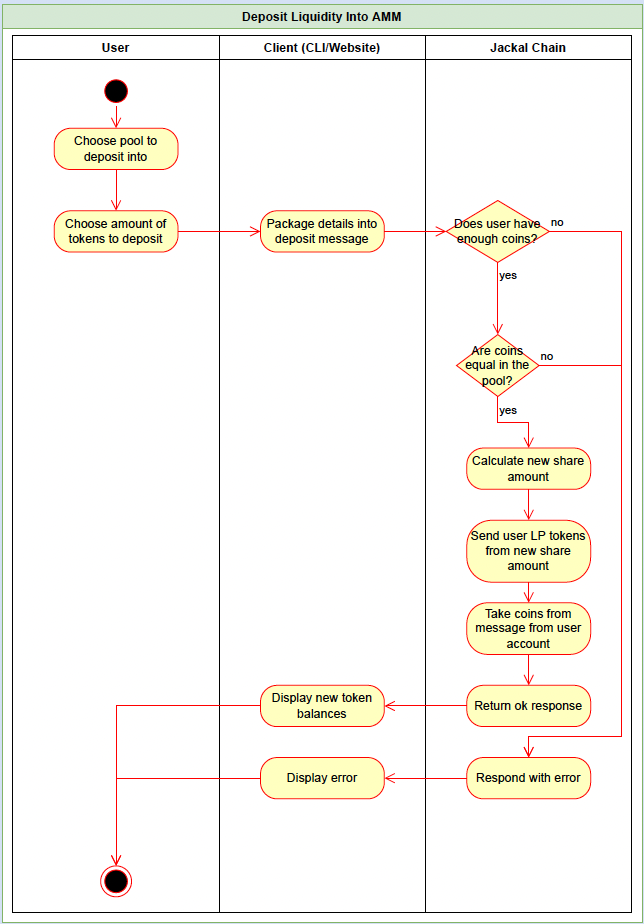
\includegraphics[width=0.5\textwidth]{assets/lp2.png}
\caption{}
\end{figure}

\begin{figure}[!htbp]
\centering
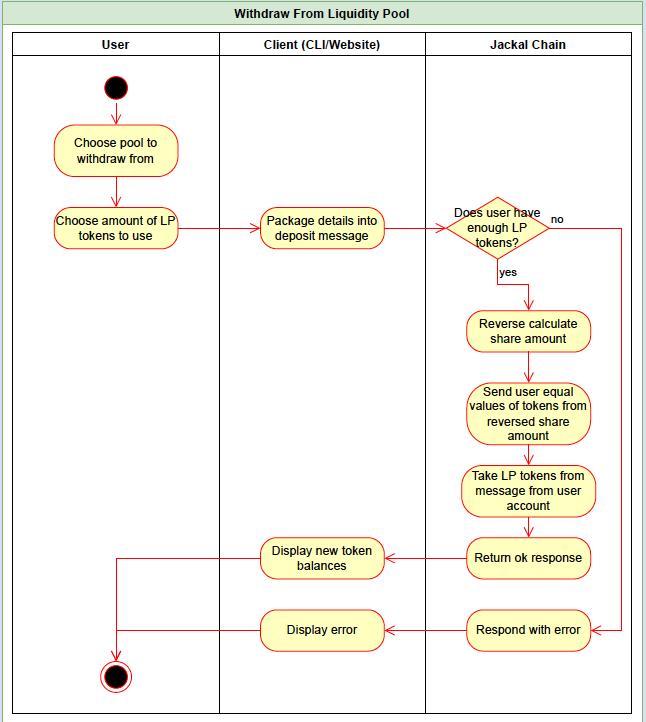
\includegraphics[width=0.5\textwidth]{assets/lp3.png}
\caption{}
\end{figure}

\begin{figure}[!htbp]
\centering
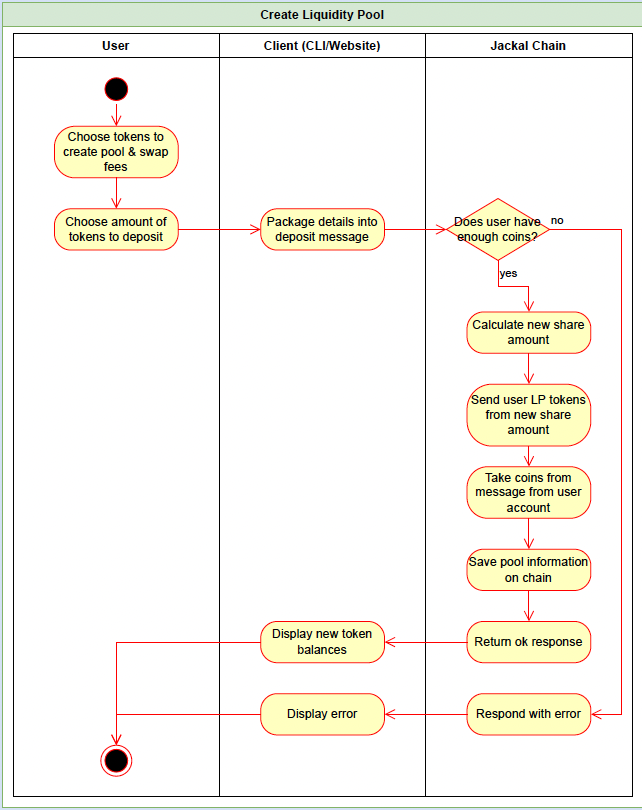
\includegraphics[width=0.5\textwidth]{assets/lp4.png}
\caption{}
\end{figure}

\begin{figure}[!htbp]
\centering
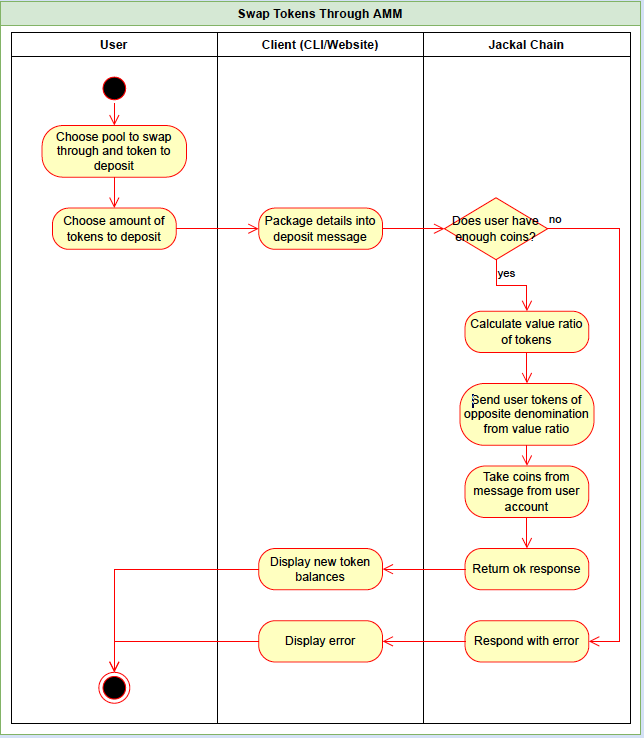
\includegraphics[width=0.5\textwidth]{assets/lp5.png}
\caption{}
\end{figure}

\newpage

\subsubsection{RNS}
The RNS module is a name service that allows users to manage human-readable names when interacting with the Jackal Blockchain and other cosmos blockchains. Users can register names, list names for sale, buy names on the marketplace, and place/accept bids from other users on their names.

\begin{figure}[!htbp]
\centering
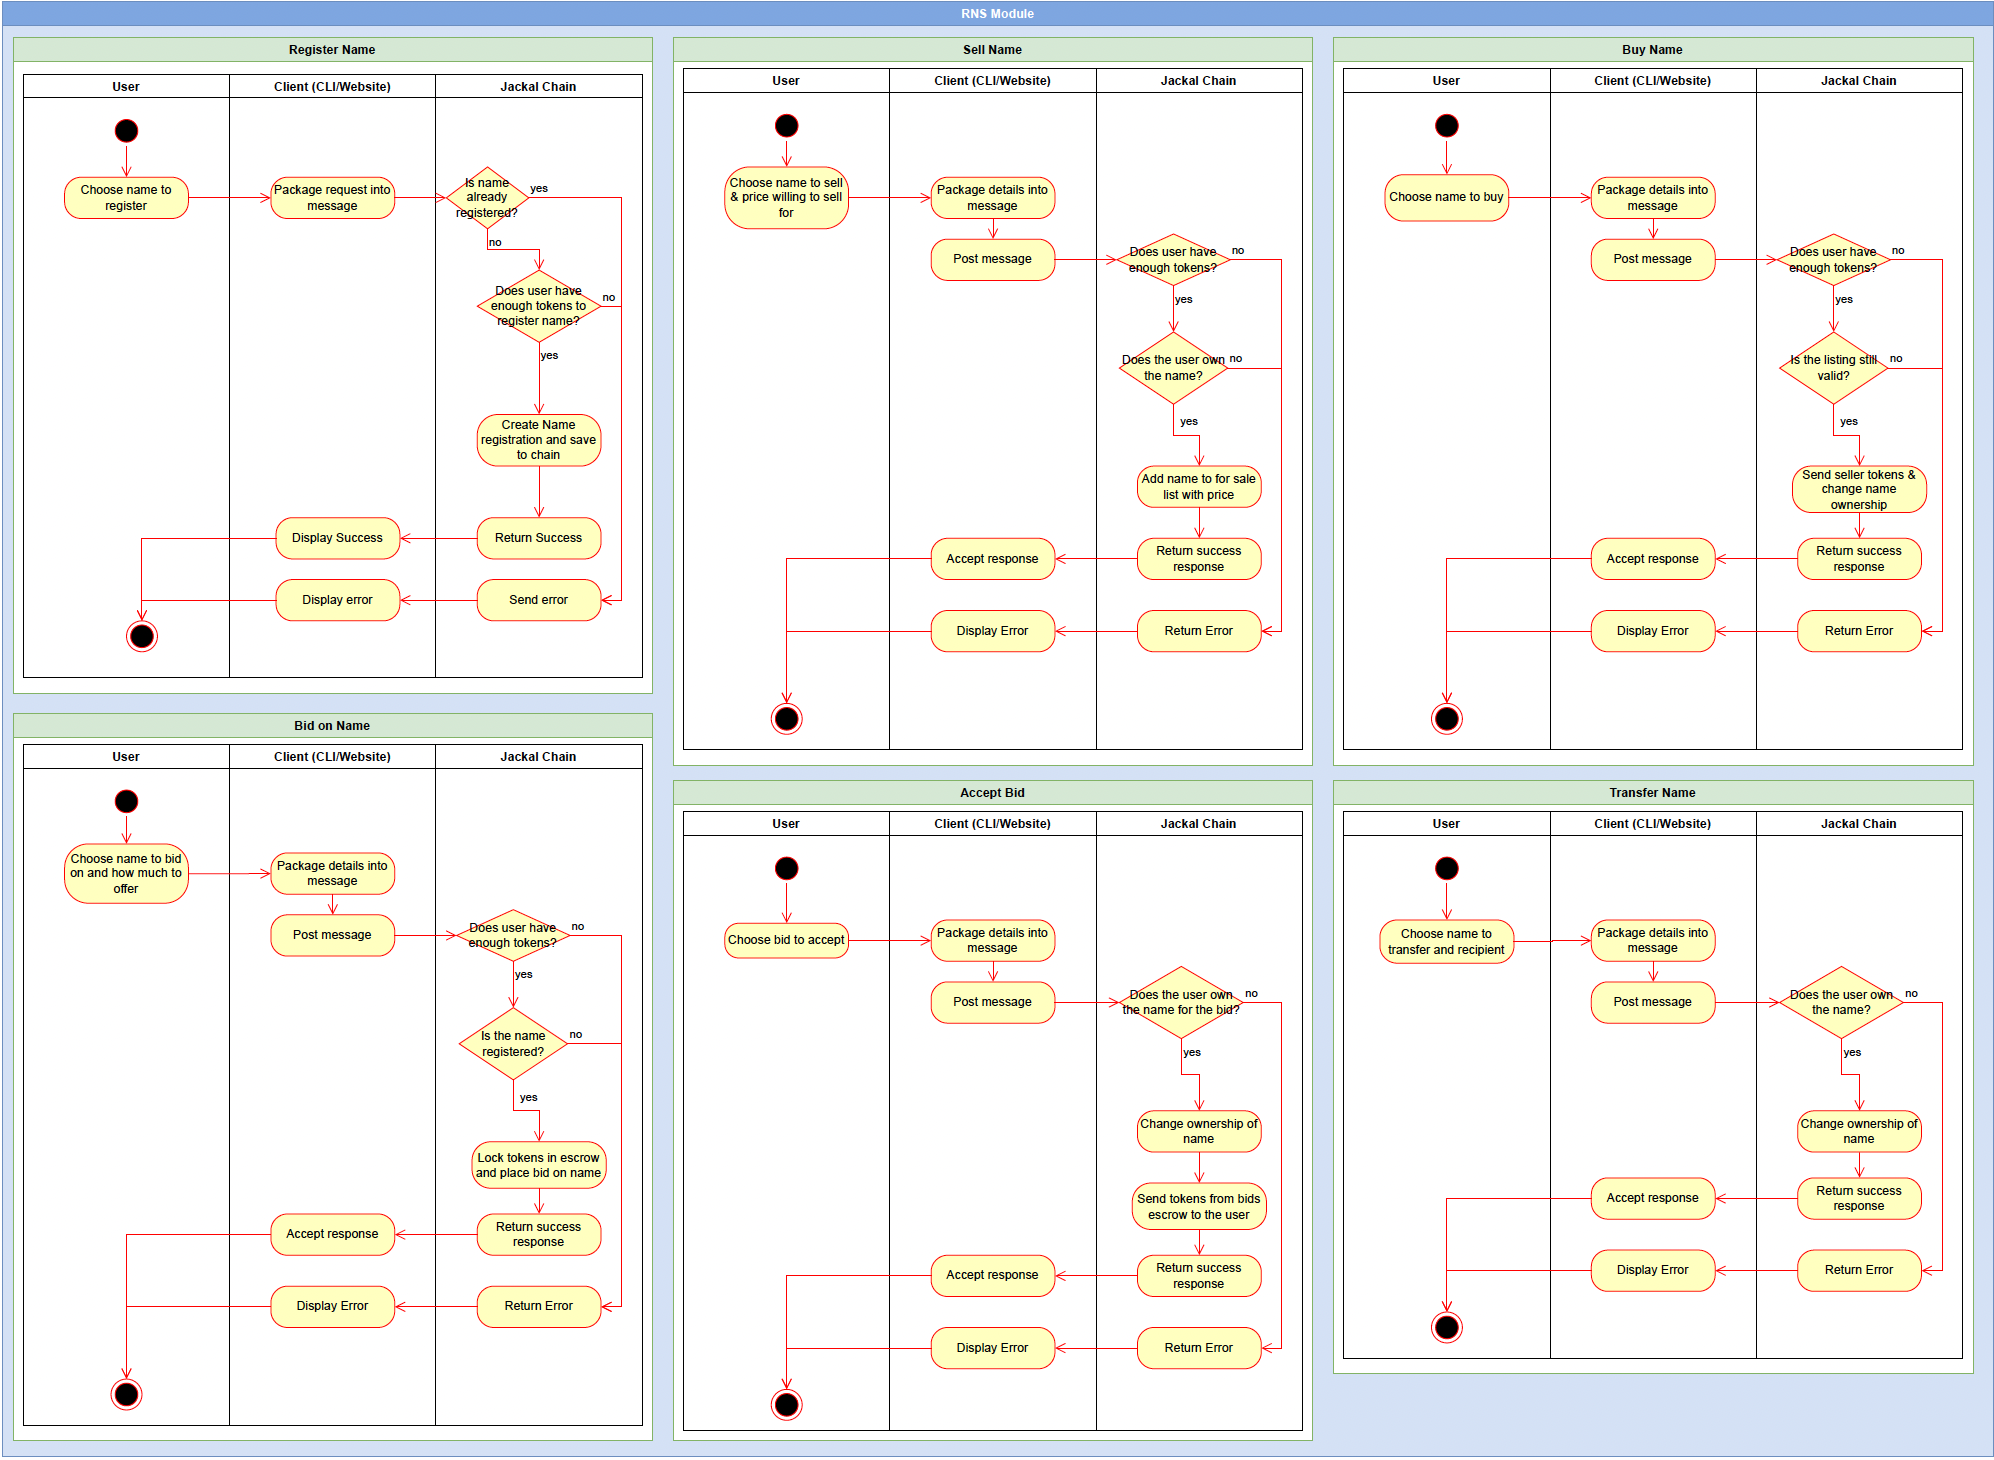
\includegraphics[width=0.7\textwidth]{assets/rns1.png}
\caption{}
\end{figure}

\begin{figure}[!htbp]
\centering
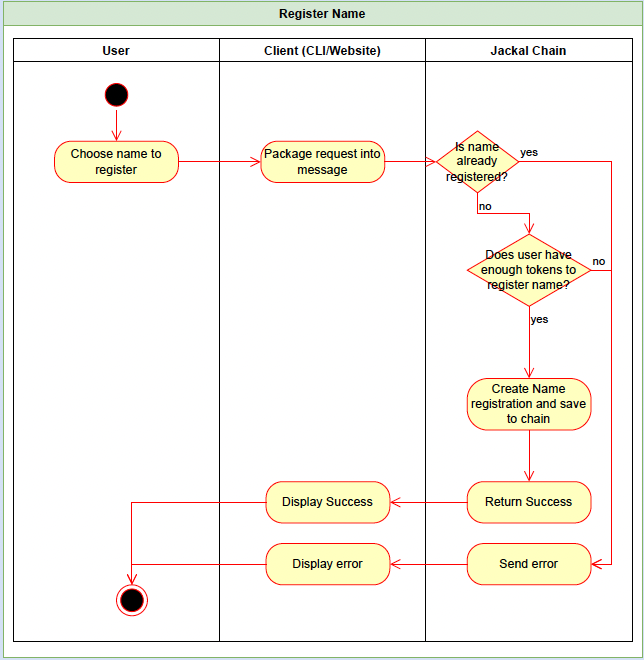
\includegraphics[width=0.5\textwidth]{assets/rns2.png}
\caption{}
\end{figure}

\begin{figure}[!htbp]
\centering
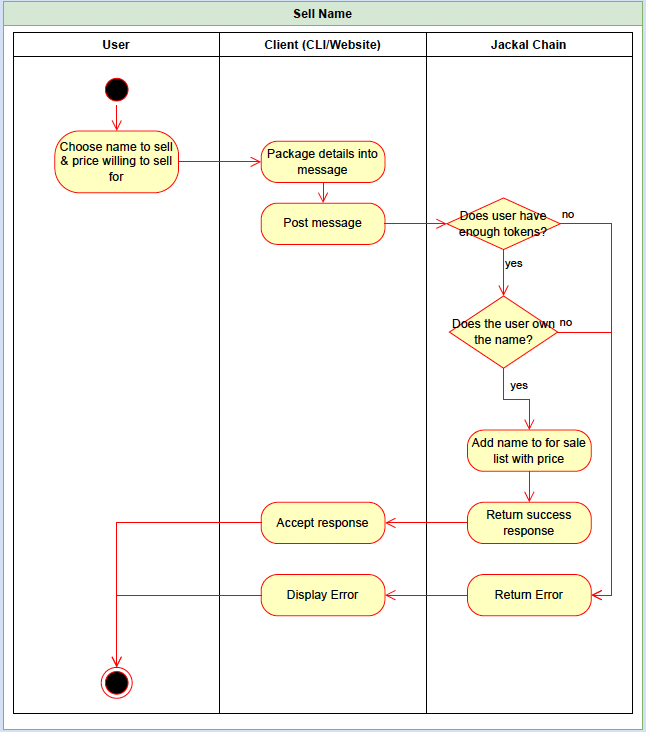
\includegraphics[width=0.5\textwidth]{assets/rns3.png}
\caption{}
\end{figure}

\begin{figure}[!htbp]
\centering
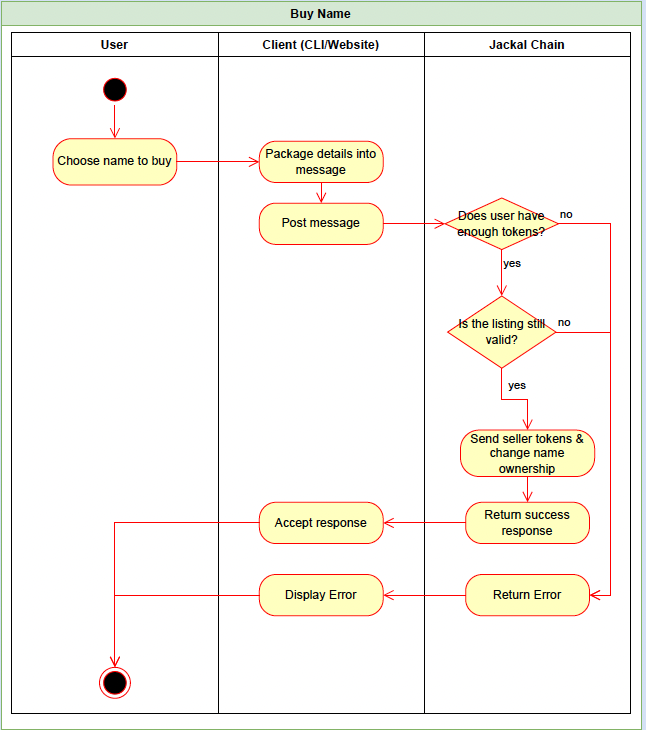
\includegraphics[width=0.5\textwidth]{assets/rns4.png}
\caption{}
\end{figure}

\begin{figure}[!htbp]
\centering
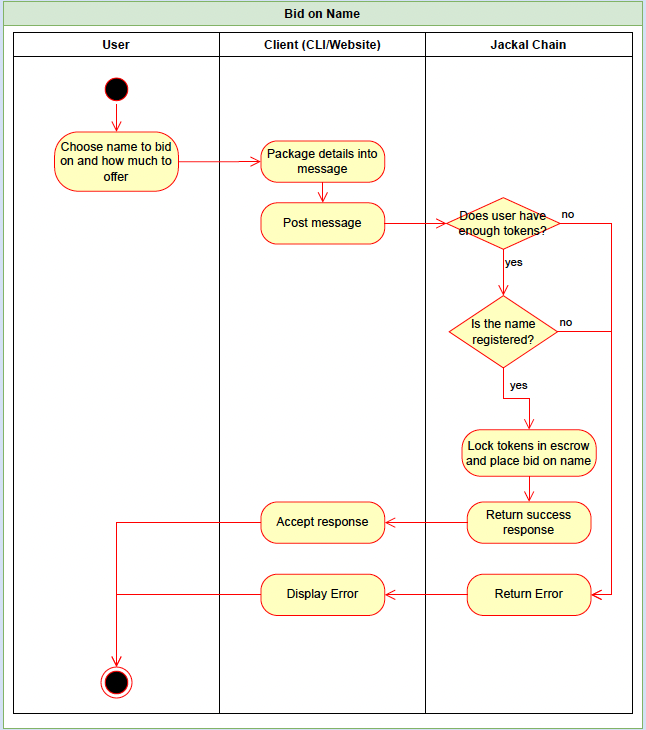
\includegraphics[width=0.5\textwidth]{assets/rns5.png}
\caption{}
\end{figure}

\begin{figure}[!htbp]
\centering
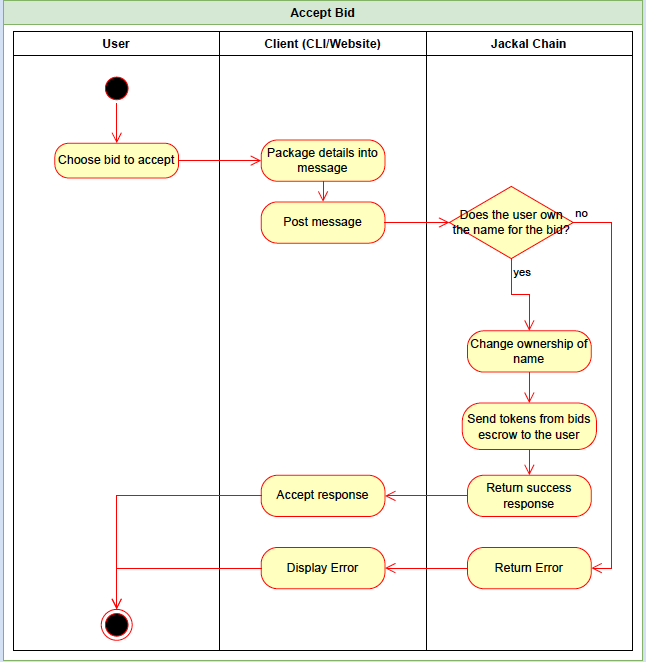
\includegraphics[width=0.5\textwidth]{assets/rns6.png}
\caption{}
\end{figure}

\begin{figure}[!htbp]
\centering
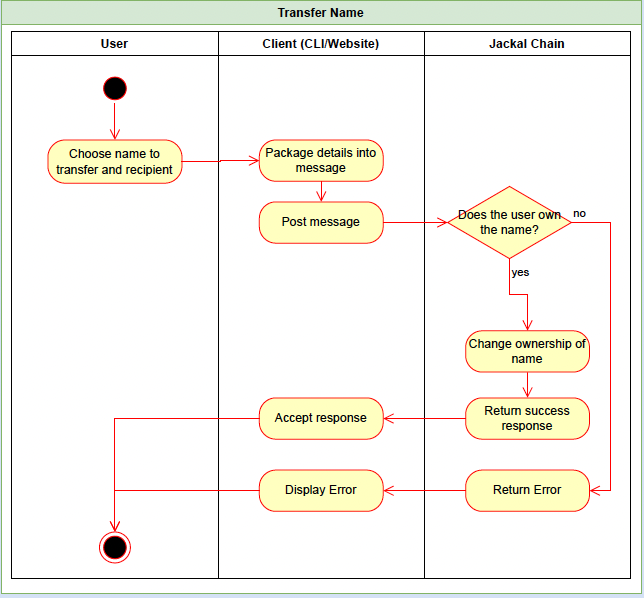
\includegraphics[width=0.5\textwidth]{assets/rns7.png}
\caption{}
\end{figure}

\newpage
\subsubsection{WASM}
Jackal incorporates the CosmWasm \cite{cosmwasm} smart contracting platform built for the Cosmos Ecosystem. The primary programming language used in this module is Rust for building secure and multi-chain smart contracts. Yet, any language that can be compiled into WASM can be supported as they become available. 

\subsubsection{Storage}
Jackal Storage is the module on-chain that determines the challenge windows \& determines the validity of proofs relating to the Jackal Proof-of-Persistence (JPOP) Protocol. It also acts as a discovery layer, similar to IPFS's Distributed Hash Tables (DHTs), allowing users to query a file and find the provider currently hosting it. \cite{dht}
\begin{figure}[!htbp]
\centering
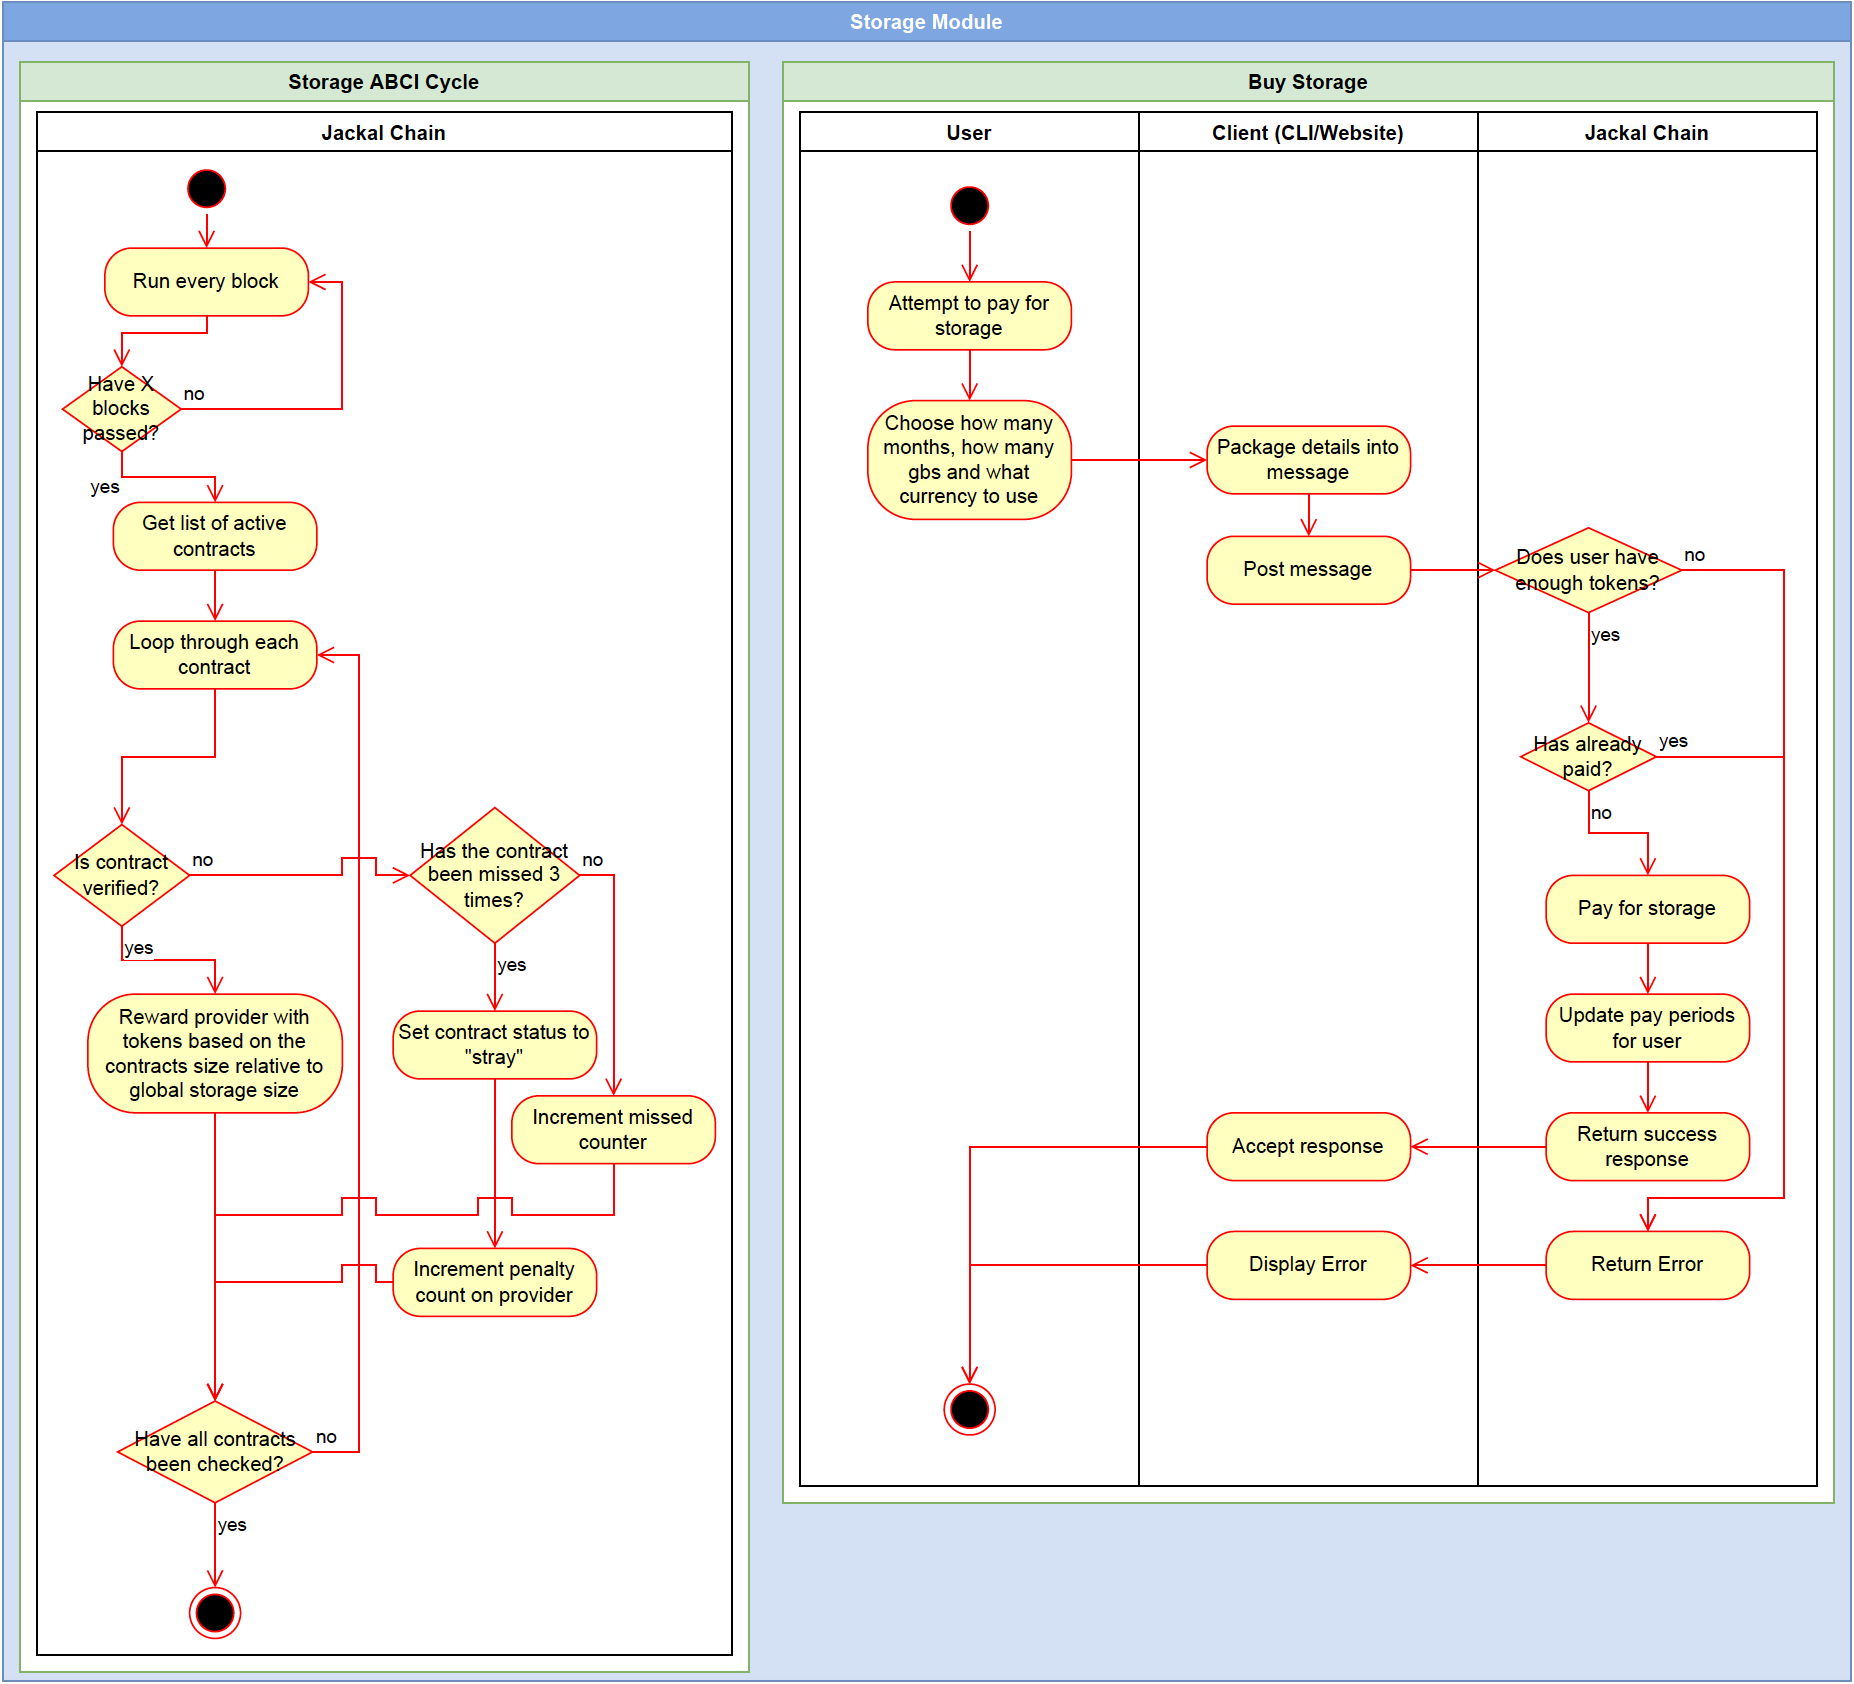
\includegraphics[width=0.7\textwidth]{assets/storage1.png}
\caption{}
\end{figure}

\paragraph{Interaction Outline}
A user first sends a file to an available Storage Provider. A list of Storage Providers can be found on the blockchain, and providers can deny any incoming request if they wish not to store new files. After receiving the entire file, the Storage Provider keeps that file in memory and posts a contract to the blockchain. If the sender does not sign the contract in X blocks (configurable by the Storage Provider), then the file is removed from memory, and the contract is burned. However, if the user within the given blocks signs the contract, the file is committed to the Storage Provider's hard storage, and the challenge windows start being created for an active contract.

\subsubsection{dSig}
The dSig module is a digital signature service that allows users to collect signatures from multiple registered users on the Jackal Blockchain. Users can create 'forms' associated with a unique file stored on Jackal and add signees (users) to collect their signatures. The signees have the following options to respond: Approve, Deny, Abstain, and No Response (Default). The form can execute a custom function after all users have voted to Approve the form.

\begin{figure}[!htbp]
\centering
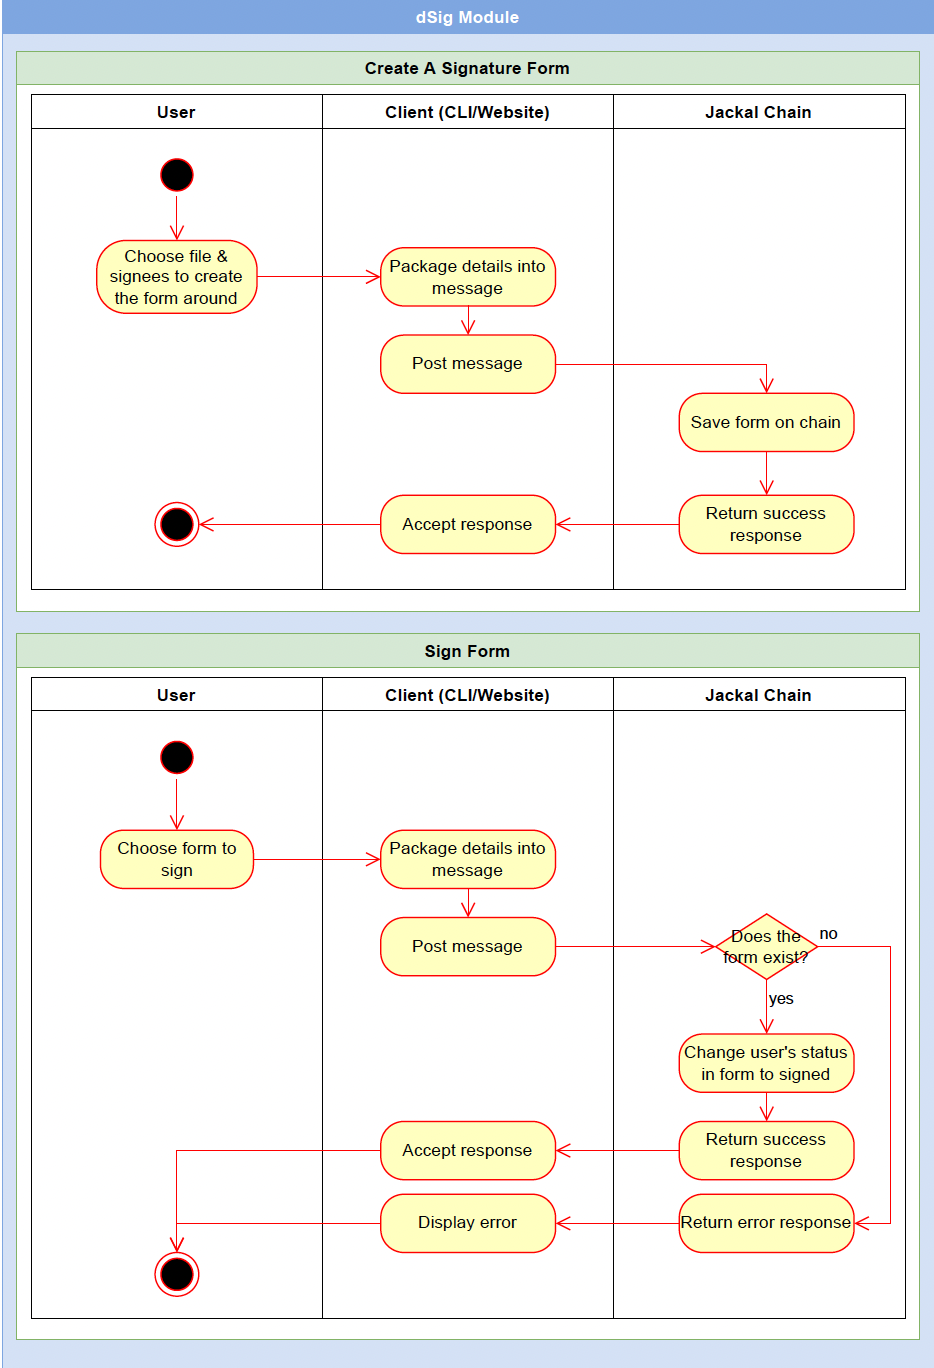
\includegraphics[width=0.7\textwidth]{assets/dsig.png}
\caption{}
\end{figure}

\newpage
\subsubsection{File Tree}
\paragraph{Intro}
The File Tree module is responsible for keeping records of a user's files and organizing them in a way that is accessible. When a user uploads a file using the Storage module, the file is only accessible from the File ID (FID) which makes the process clunky and obtuse to remember every file uploaded to Jackal. Furthermore, every single upload would be required to be public, or the user would need to keep track of every symmetric key used to encrypt the files and manually map them to the FIDs. The solution to this is a tree structure storing each file as an entry in the tree. Organizing this structure is also trivial as we can assign children to pseudo files that we call folders. Finally to keep track of encryption keys, the protocol maps every file to its respective key.

\begin{figure}[!htbp]
\centering
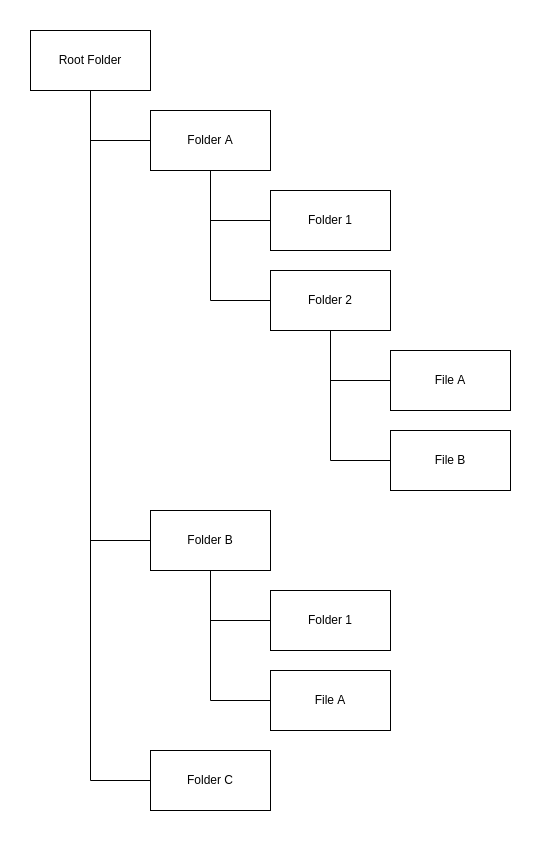
\includegraphics[width=0.4\textwidth]{assets/filetree1.png}
\caption{}
\end{figure}

\paragraph{Folder Abstraction}
These, of course, are all abstractions of what's actually under the hood. The File Tree module doesn't actually handle any of the folder logic, the system believes it is storing files that act as metadata stores, which then update to reflect changes in folders. This gives the user experience the feeling that folders and files are separate entities in the tree, but in reality they are identical.

\paragraph{File Entry Structure}
Storing file entries on-chain is a hurdle being that the chain itself is public. This requires the use of client-side encryption before uploading data to the chain itself. The main component of a file is a location (Address), allowing users to query the rest of the data from the file. You can think of the location as a key in a traditional key-value store or a path in bucket-based storage. The address is hashed using SHA256 to ensure it is impossible to retrieve the plain-text representation of the file name, while still being able to query the file using its given name. 

\begin{figure}[!htbp]
\centering
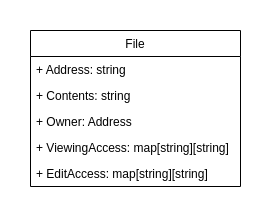
\includegraphics[width=0.4\textwidth]{assets/filetree2.png}
\caption{}
\end{figure}

\newpage
The second most important data point in a file is the content of the file, this field is extremely versatile as it can store any string. Traditionally this is used to store a JSON list of FIDs to point to a file on the Storage Module, however, the protocol can also theoretically use it to store short bits of text like encrypted passwords for a private password manager. The owner tag is a hashed version of the owner hiding what address owns each file, this field can be changed to reflect the transferral of ownership. When making changes to the file such as deletion, movement or adding/removing viewers/editors, the owner field is consulted to determine permissions. The same applies to edit access, editors can update the contents but nothing else. 

\paragraph{Encrypted Viewing Access}
For users to view files, they need access to the symmetric keys used to encrypt the files. To do this, the protocol has a map of hashed addresses with each user's respective version of the symmetric key encrypted with that address's corresponding public key. The protocol can then store that map in the file entry to act as an encryption key discovery layer. The addresses in this viewing list are only able to access files and decrypt the data in their client, they have no privileges over the modification of the file entry in any way.

\begin{figure}[!htbp]
\centering
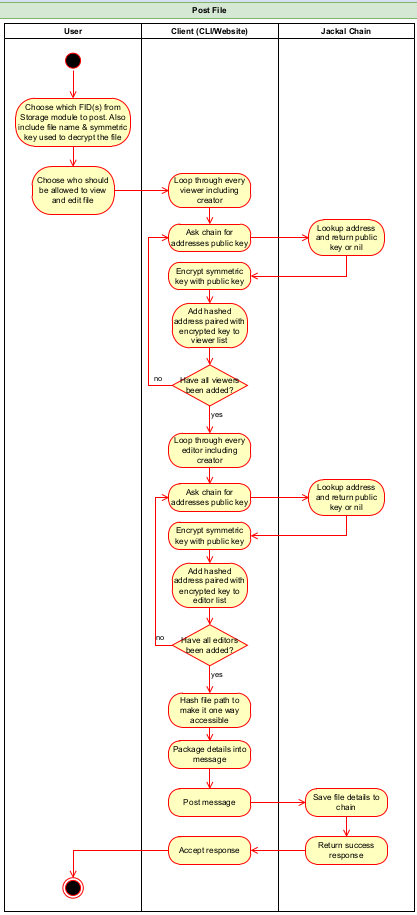
\includegraphics[width=0.6\textwidth]{assets/filetree3.png}
\caption{}
\end{figure}

\begin{figure}[!htbp]
\centering
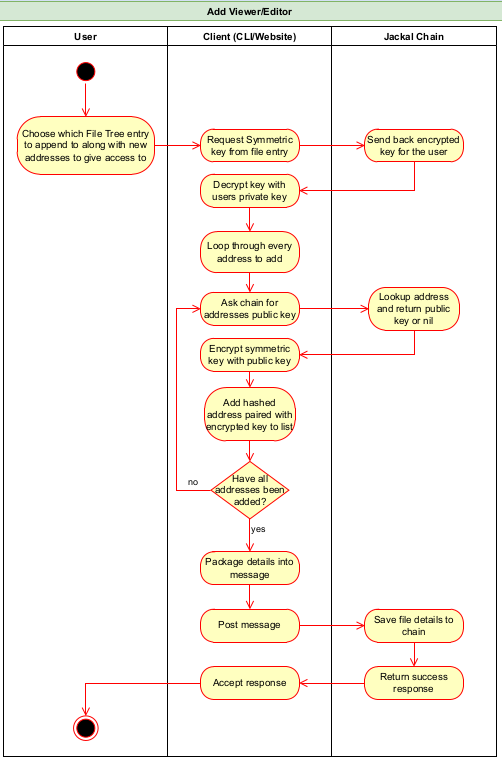
\includegraphics[width=0.6\textwidth]{assets/filetree4.png}
\caption{}
\end{figure}

\begin{figure}[!htbp]
\centering
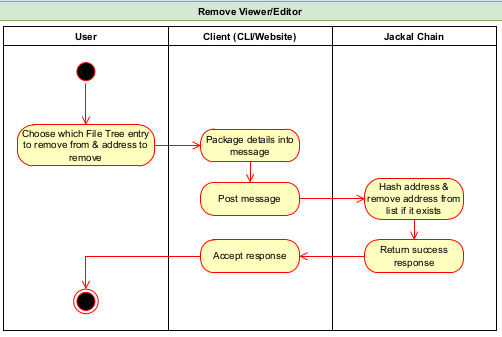
\includegraphics[width=0.6\textwidth]{assets/filetree5.png}
\caption{}
\end{figure}

\begin{figure}[!htbp]
\centering
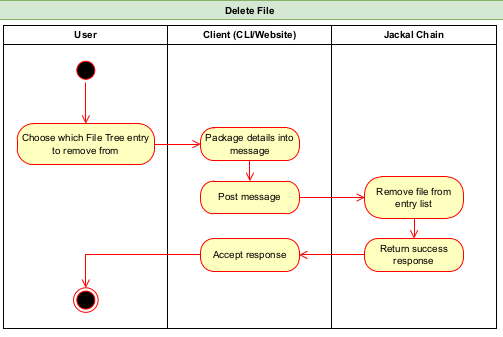
\includegraphics[width=0.6\textwidth]{assets/filetree6.png}
\caption{}
\end{figure}

\begin{figure}[!htbp]
\centering
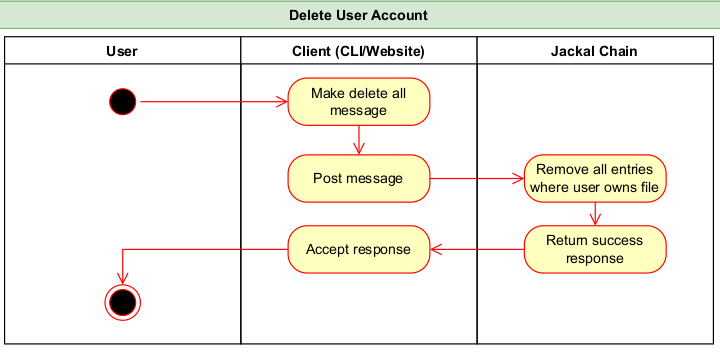
\includegraphics[width=0.6\textwidth]{assets/filetree7.png}
\caption{}
\end{figure}

\begin{figure}[!htbp]
\centering
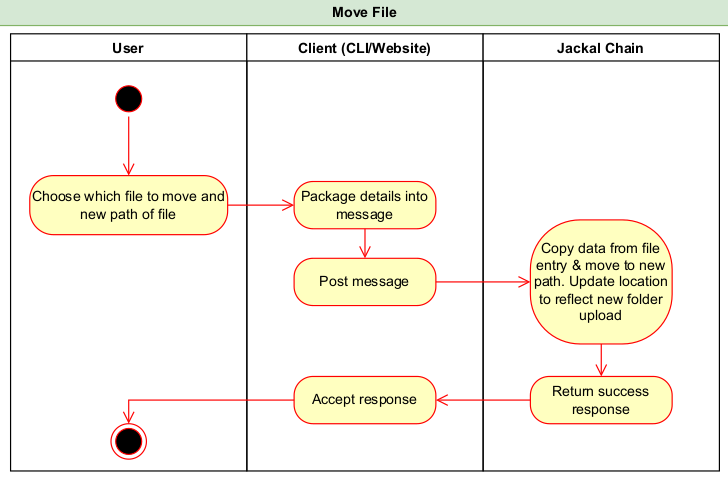
\includegraphics[width=0.6\textwidth]{assets/filetree8.png}
\caption{}
\end{figure}

\begin{figure}[!htbp]
\centering
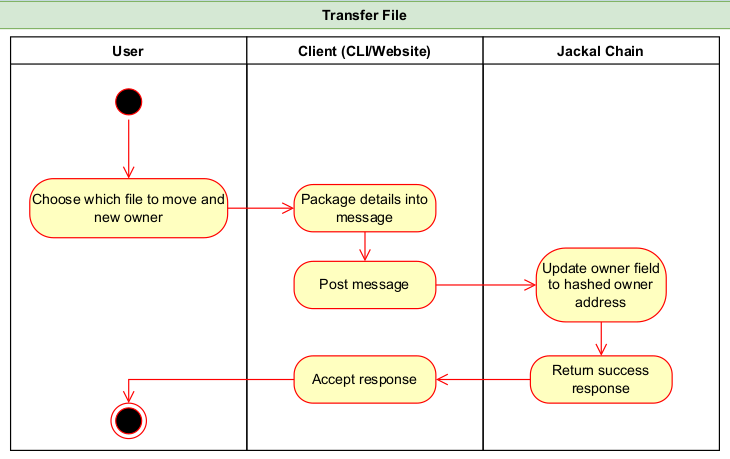
\includegraphics[width=0.6\textwidth]{assets/filetree9.png}
\caption{}
\end{figure}

\newpage
\subsection{Storage Providers}
A Jackal Storage Provider is a dedicated web server optimized for data storage that accepts incoming files from users and creates contracts for the users to approve. These contracts last until the user either cancels them, or the provider itself goes offline.

\begin{figure}[!htbp]
\centering
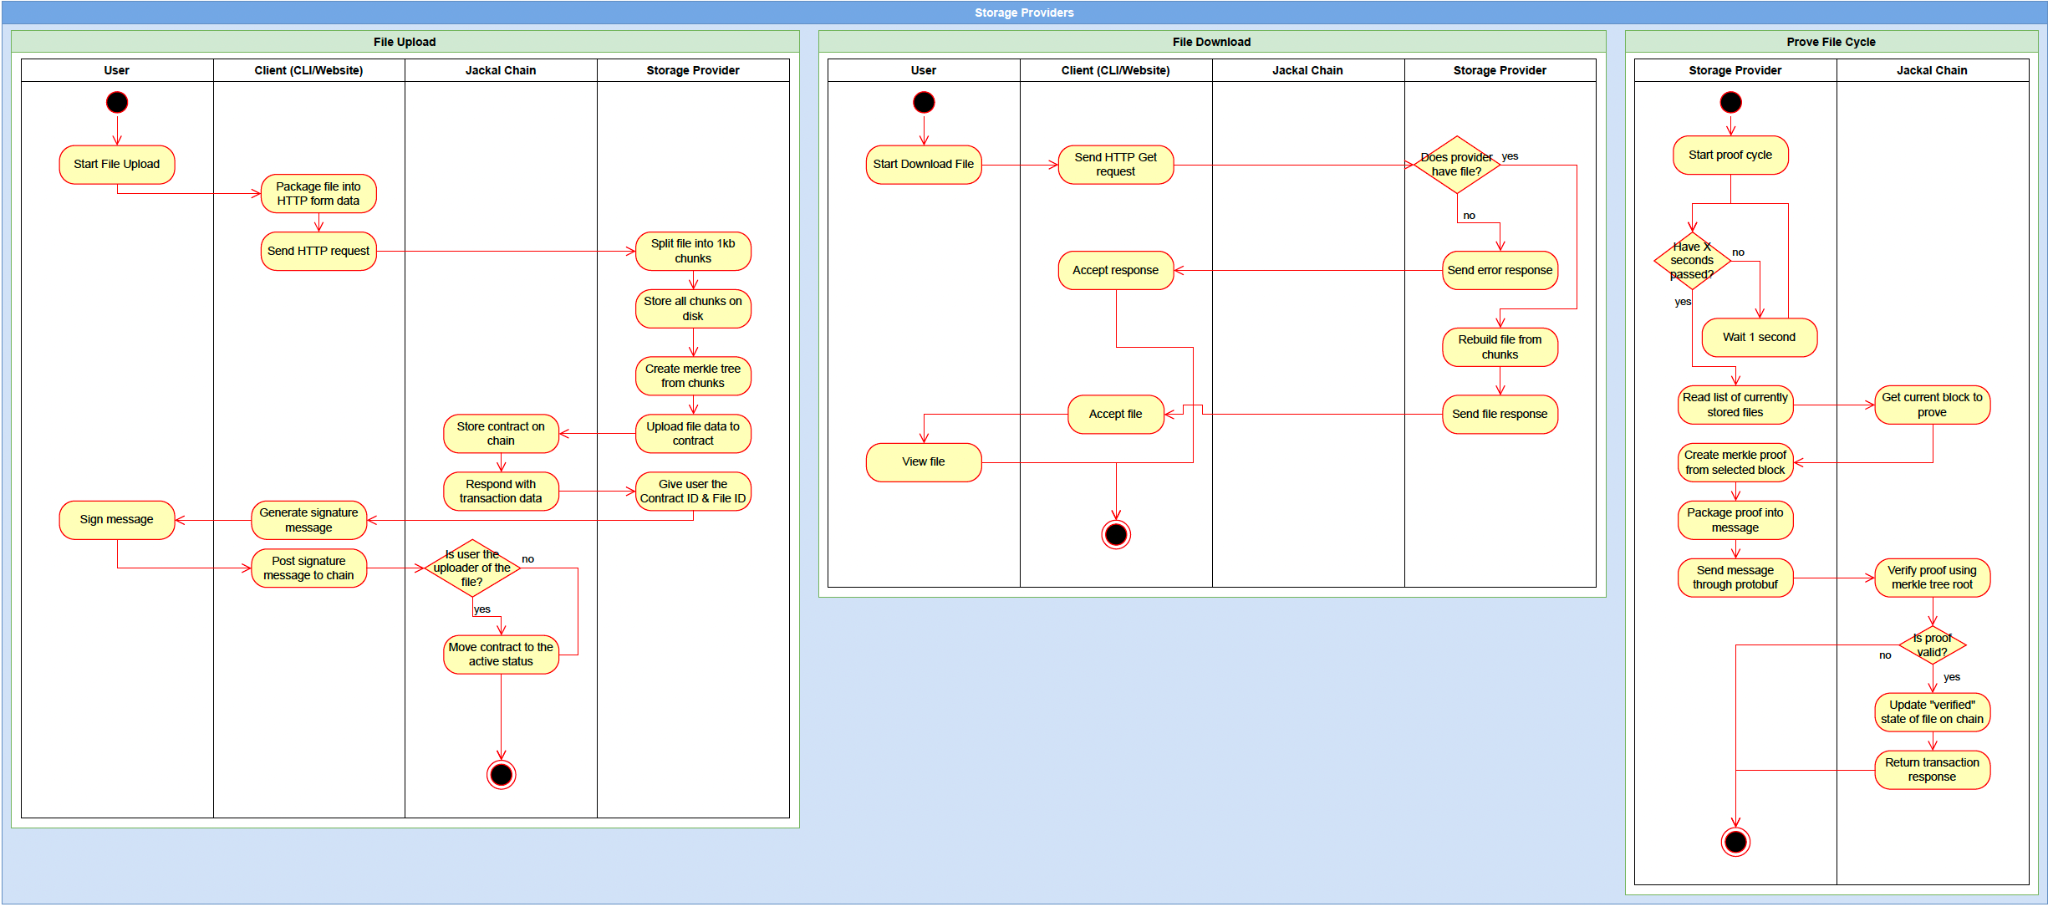
\includegraphics[width=0.8\textwidth]{assets/providers1.png}
\caption{}
\end{figure}

\begin{figure}[!htbp]
\centering
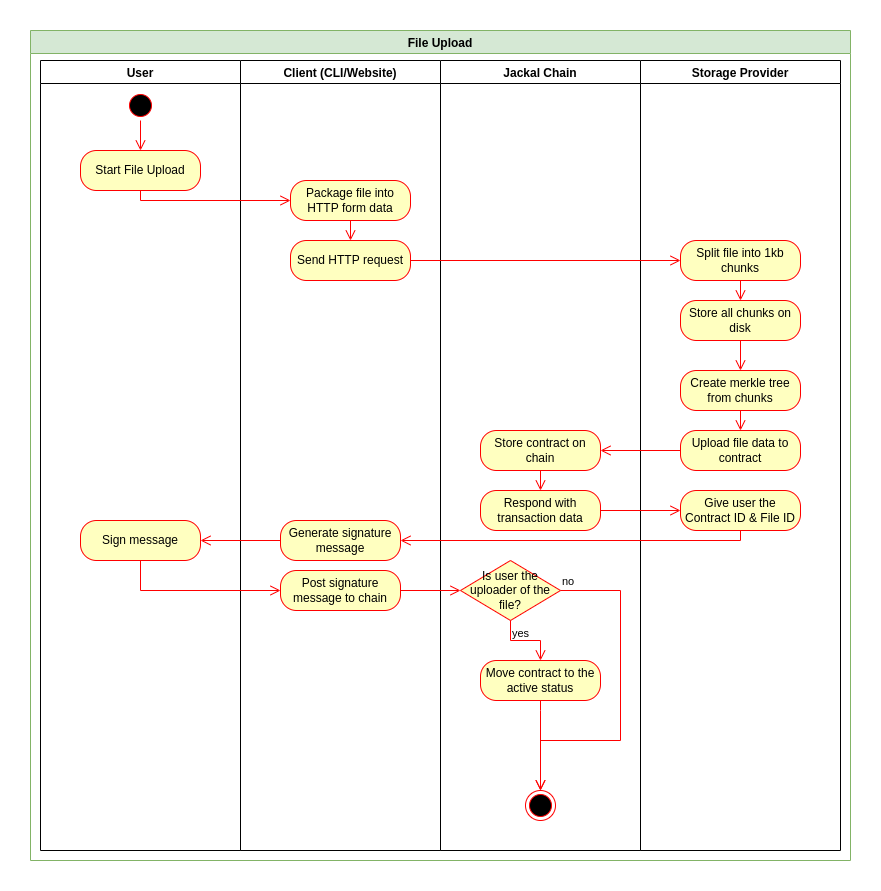
\includegraphics[width=0.6\textwidth]{assets/providers2.png}
\caption{}
\end{figure}

\begin{figure}[!htbp]
\centering
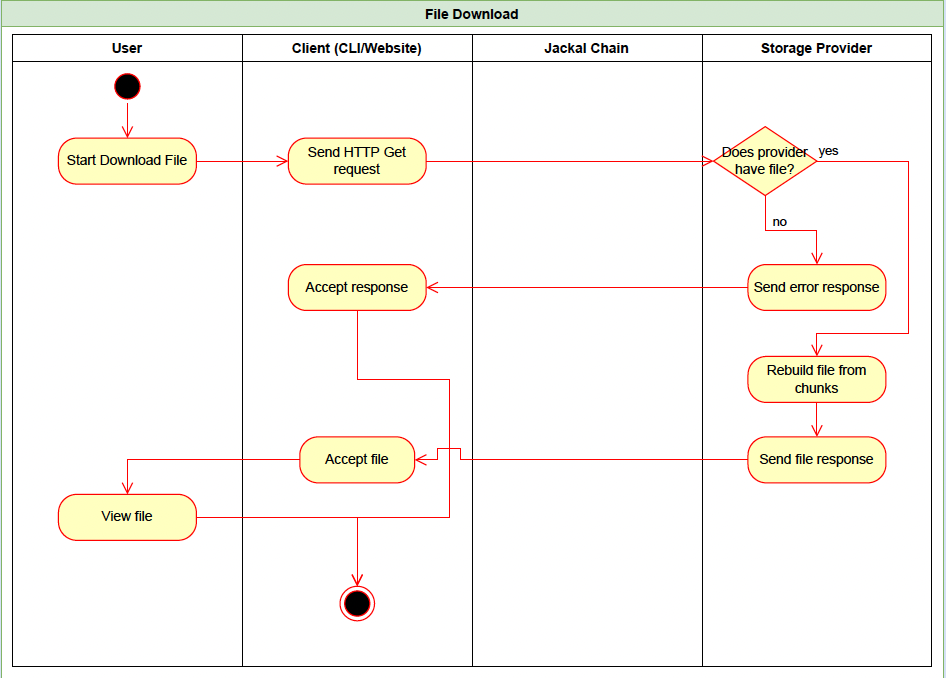
\includegraphics[width=0.6\textwidth]{assets/providers3.png}
\caption{}
\end{figure}

\begin{figure}[!htbp]
\centering
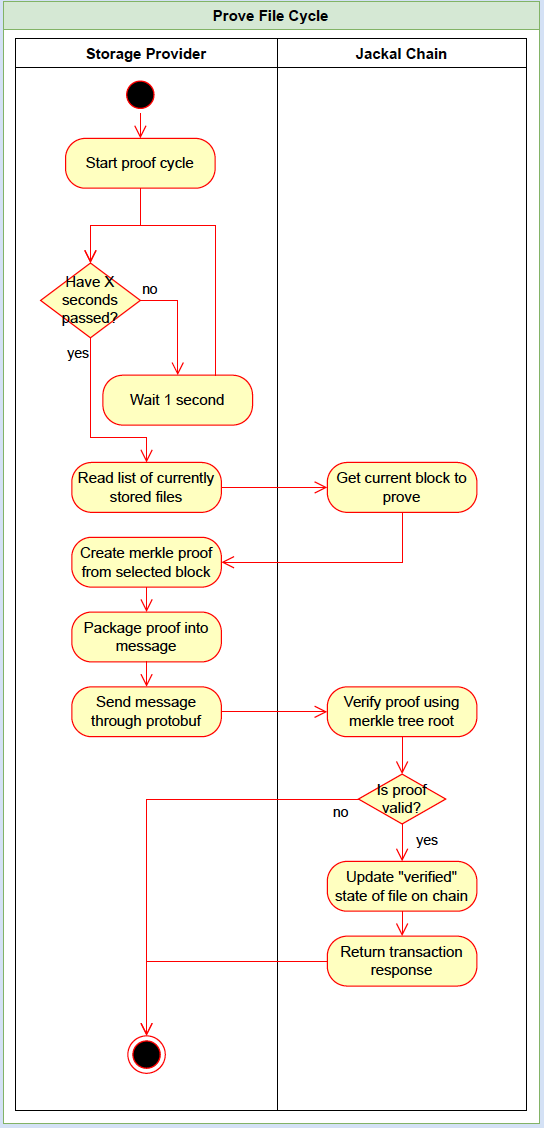
\includegraphics[width=0.5\textwidth]{assets/providers4.png}
\caption{}
\end{figure}

\newpage
\subsection{Validators}
The Jackal Validators are web servers that are secure, dedicated machines that participate in the consensus protocol by broadcasting cryptographic signatures, or votes, to agree upon the next block. Voting power is determined by the amount of staking tokens delegated by non-validators and bonded as collateral to earn a reward. These non-validators, or delegators, incur the risk of getting punished (slashed) if the delegate validator gets hacked or violates the protocol.

\subsection{Tokens}
\subsubsection{JKL}
JKL is the native inflationary token that powers the Jackal Protocol. This token provides utility to the protocol in the following ways. 

\paragraph{dApps}
Applications built leveraging the Jackal Protocol, such as Jackal Storage and the RNS Marketplace, may choose to include the JKL token to expand its utility. 

\paragraph{Securing the Network}
As the Jackal Protocol is a Proof-of-Stake (PoS) Cosmos L1 blockchain, JKL can be delegated to validators to secure the network and earn JKL rewards. Otherwise known as staking or staked tokens.

\paragraph{Transaction Fees}
Transactions on the Jackal Protocol must be paid for using JKL. As the protocol is PoS, the cost of transactions is inexpensive. 

\paragraph{Governance}
Tokens bonded with Validators grant on-chain governance participation within the Jackal Protocol to vote on text, software, spending, and other governance proposals. 

\paragraph{Collateral}
The JKL token can act as collateral for validators, storage providers, and other smart contract use cases. 

\paragraph{Liquidity Provision}
JKL can be allocated into a liquidity pool to earn rewards. 

\subsubsection{JWL}
JWL is the second native token to the Jackal Protocol. JWL tokens are immutable, meaning that there is a finite number of tokens that will be minted at the genesis of the Jackal Protocol. At genesis, there is no utility for the JWL token, and these tokens should be treated as such. 

\section{Use Cases}
The Jackal Labs team will launch six decentralized applications to feature the power of the Jackal Protocol at genesis. Jackal Storage is a self-custodial and private cloud data storage product. Retriever Name Service is an inter-blockchain communication name service for the entire Cosmos ecosystem for seamless organization and efficiency when using multiple blockchains. Jackal Web Hosting is a fully open HTTP gateway for static websites on Jackal Storage. Jackal Swap is a decentralized token exchange for Cosmos-based tokens. Jackal Sign is a digital signature service that allows users to collect signatures from Jackal users. Jackal Manager is a decentralized password manager for web2 applications built with the Jackal Wallet and Jackal Storage. 

Additional decentralized applications can be created by the Jackal Community using CosmWasm smart contracts. 

\section{Acknowledgements}
Many individuals should be acknowledged for their contributions and tireless efforts in building this protocol over the last 11 months. Those acknowledged include; Marston Connell, Patrick Dunlop, Erin Rivas, Will Grant, Bi Phan, Emory Wesson, Danny Ahn, Justin Nguyen, and Max Pochapski. 

\newpage
\printbibliography %Prints bibliography

\end{document}